\begin{center}
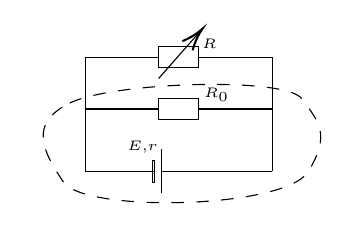
\begin{tikzpicture}[x=0.75pt,y=0.75pt,yscale=-1,xscale=1]
%uncomment if require: \path (0,300); %set diagram left start at 0, and has height of 300

%Shape: Battery [id:dp2916012360245832] 
\draw   (262.5,144) -- (276,144) (279,133.36) -- (279,154.64) (279,144) -- (292.5,144) (274.8,138.68) -- (276,138.68) -- (276,149.32) -- (274.8,149.32) -- (274.8,138.68) -- cycle ;
%Straight Lines [id:da2734255254924993] 
\draw    (242.5,89) -- (242.5,144) ;
%Straight Lines [id:da8342089479991157] 
\draw    (332.5,89) -- (332.5,144) ;
%Straight Lines [id:da4571525926989708] 
\draw    (242.5,144) -- (262.5,144) ;
%Straight Lines [id:da08274074907134321] 
\draw    (292.5,144) -- (332.5,144) ;
%Shape: Resistor [id:dp8558892883342235] 
\draw   (277.9,109) -- (297.1,109) -- (297.1,119) -- (277.9,119) -- (277.9,109) -- cycle (272.5,114) -- (277.9,114) (297.1,114) -- (302.5,114) ;
%Straight Lines [id:da7537185022486395] 
\draw    (272.5,114) -- (242.5,114) ;
%Straight Lines [id:da8797643160506492] 
\draw    (332.5,114) -- (302.5,114) ;
%Shape: Resistor [id:dp5429151855494494] 
\draw   (277.9,84) -- (297.1,84) -- (297.1,94) -- (277.9,94) -- (277.9,84) -- cycle (272.5,89) -- (277.9,89) (297.1,89) -- (302.5,89) ;
%Straight Lines [id:da9804503401878168] 
\draw    (272.5,89) -- (242.5,89) ;
%Straight Lines [id:da5427185273385342] 
\draw    (332.5,89) -- (302.5,89) ;
%Straight Lines [id:da37813397906193025] 
\draw    (277.81,99.32) -- (297.64,76.82) ;
\draw [shift={(298.96,75.32)}, rotate = 131.4] [color={rgb, 255:red, 0; green, 0; blue, 0 }  ][line width=0.75]    (10.93,-3.29) .. controls (6.95,-1.4) and (3.31,-0.3) .. (0,0) .. controls (3.31,0.3) and (6.95,1.4) .. (10.93,3.29)   ;
%Shape: Polygon Curved [id:ds525720693471261] 
\draw  [dash pattern={on 4.5pt off 4.5pt}] (235,111.13) .. controls (255,101.13) and (338.92,98.14) .. (346.92,109.14) .. controls (354.92,120.14) and (360.92,126.14) .. (349.92,144.14) .. controls (338.92,162.14) and (241.92,164.14) .. (231.92,149.14) .. controls (221.92,134.14) and (215,121.13) .. (235,111.13) -- cycle ;

% Text Node
\draw (264.5,127.05) node [anchor=north west][inner sep=0.75pt]   [align=left] {$ $};
% Text Node
\draw (261.5,128) node [anchor=north west][inner sep=0.75pt]  [font=\tiny] [align=left] {$\displaystyle E$,$\displaystyle r$};
% Text Node
\draw (298.5,102.55) node [anchor=north west][inner sep=0.75pt]  [font=\tiny] [align=left] {$\displaystyle R_{0}$};
% Text Node
\draw (297.5,79.05) node [anchor=north west][inner sep=0.75pt]  [font=\tiny] [align=left] {$\displaystyle R$};
\end{tikzpicture}

\end{center}